\section{Kapitel 1 - Einführung in BWL}
\subsection{Übersicht}
\underline{BWL:} Beschreibt das Wirtschaften in Betrieben\\
\underline{Wichtige Personen in der BWL:}
\begin{itemize}
  \item[Schmalenbach] \nl BWL als Kunstlehre
  \item[Nicklisch] \nl Dienst an der Gemeinschaft
  \item[Rieger] \nl Streben nach Gewinn
  \item[Gutenberg] \nl Betriebe werden in der Gesamtheit ihrer Funktion betrachtet.
                   Gilt als Begründer der der modernen deutschen BWL.
\end{itemize}
\subsection{Prinzipen der BWL}
\begin{description}
  \item[Ökonomisches Prinzip] \nl Streng Methodische Eindimensionalität durch Konzentration
                auf die \emph{wirtschaftliche} Seite.
  \item[Systemorientiertes Prinzip] \nl Unternehmen werden als zweckgebundenes soziales System aufgefasst (multidimensional).
                                    $\rightarrow$ BWL als Führungslehre (Management)
  \item[Maximalprinzip (Mengen) $\Leftrightarrow$ Budgetprinzip (Geld) ] \nl max. Ertrag $\rightarrow$ geg. Einsatz
  \item[Minimalprinzip (Mengen) $\Leftrightarrow$ Sparprinzip (Geld)] \nl geg. Ertrag $\rightarrow$ min. Einsatz
\end{description}
\subsection{Produktionsfaktoren}
\begin{itemize}
  \item Elementarfaktoren\nl Elementarfaktoren mit unmittelbaren Bezug zum Produktionsobjekt (Arbeitsleistung, Betriebsmittel, Werkstoffe)
  \item[\textbullet Dispositive Faktoren]\nl Bezeichnet leitende Arbeiten (Geschäftsleitung, Planung \& Organisation, Kontrolle)
  \item[\textbullet Originäre Faktoren]\nl Ursprünglich notwendig für einen Betrieb
  \item[\textbullet Derivative Faktoren]\nl Um den Betrieb zum laufen zu bringen, braucht man diese (Planung, Kontrolle)
\end{itemize} 

\subsection{Unternehmensgrößenklassen der EU}
\begin{tabular}{|l|| c|c|c|}
  \hline
  Unternehmensgröße & Mitarbeiter & Umsatz & Bilanzsumme \\
  \hline
  klein & bis 49 & bis 10Mio. & bis 10Mio \\
  mittel & bis 249 & bis 50Mio. & bis 43Mio \\
  groß & ab 250 & ab 50Mio. & ab 43Mio \\
  \hline
\end{tabular}\\
Ein Unternehmen wird einer dieser Klassen zugeordnet, wenn 2 der 3 Merkmale gegeben sind.


%Tree Einzelwirtschaft
\subsection{Zusammenhänge Einzelwirtschaft}
\tikzstyle{level 1}=[level distance=5cm, sibling distance=2cm]
\tikzstyle{level 2}=[level distance=5cm, sibling distance=1cm]
\tikzstyle{bag} = [text width=4em, text centered]
\tikzstyle{end} = [circle, minimum width=3pt,fill, inner sep=0pt]
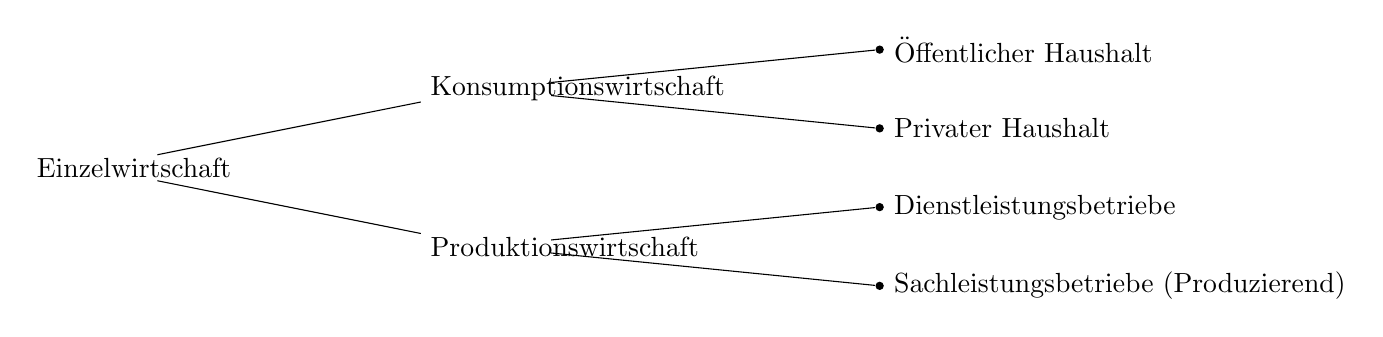
\begin{tikzpicture}[grow=right, sloped]
\node[bag] {Einzelwirtschaft}
    child {
        node[bag] {Produktionswirtschaft}        
            child {
                node[end, label=right:
                    {Sachleistungsbetriebe (Produzierend)}] {}
                edge from parent
                node[above] {}
                node[below]  {}
            }
            child {
                node[end, label=right:
                    {Dienstleistungsbetriebe}] {}
                edge from parent
                node[above] {}
                node[below]  {}
            }
            edge from parent 
            node[above] {}
            node[below]  {}
    }
    child {
        node[bag] {Konsumptionswirtschaft}        
        child {
                node[end, label=right:
                    {Privater Haushalt}] {}
                edge from parent
                node[above] {}
                node[below]  {}
            }
            child {
                node[end, label=right:
                    {Öffentlicher Haushalt}] {}
                edge from parent
                node[above] {}
                node[below]  {}
            }
        edge from parent         
            node[above] {}
            node[below]  {}
    };
\end{tikzpicture}


\subsection{Zielarten}
\begin{itemize}
  \item \textbf{Wirtschaftsbezug}: Ökonomische Ziele, Nichtökonomische Ziele
  \item \textbf{Geldbezug}: Monetäre Ziele, Nichtmonetäre Ziele
  \item \textbf{Leistungsbezug}: Sachziele, Formalziele
  \item \textbf{Umweltbezug}: Ökologische Ziele, Nichtökologische Ziele 
\end{itemize}
